\documentclass[a4paper,11pt,fleqn,twoside,openright]{memoir}

%%%%%%%%%%%%%%%%%%%%%%%%%%
%% COMMAND DEACTIVATION %%
%%%%%%%%%%%%%%%%%%%%%%%%%%

\let\added\undefined
\let\deleted\undefined


%%%%%%%%%%%%%%
%% PACKAGES %%
%%%%%%%%%%%%%%


%%% Initial things %%%
% Fix various issues with LaTeX2e
\usepackage{fixltx2e}
% Font package
\usepackage{fourier}
% Index
\usepackage{makeidx}
\makeindex


%%% Translations and character encodings %%%
% Enable use of several characters, including æ, ø and å
\usepackage[utf8]{inputenc}
% Danish language
\usepackage[danish]{babel}
% Use PostScript fonts instead of bitmap ones. Also does other stuff.
\usepackage[T1]{fontenc}
% Various LaTeX symbols
\usepackage{latexsym}
% Wider selection of colours
\usepackage{xcolor}
% Improved element justification
\usepackage{ragged2e}
% Font improvements
\usepackage{fix-cm}
% Enables inclusion of PDF files
\usepackage{pdfpages}
% Enables various forms of lines, like double-underlining (\uuline{})
\usepackage[normalem,normalbf]{ulem}
% Sets the tolerance for distance between words, determining when to hyphenate.
\pretolerance=2500


%%% Figures and tables (Floats) %%%
% Ensures that floats won't appear -before- the place where they're added
\usepackage{flafter}
% Enable multi-rows and -columns
\usepackage{multirow}
\usepackage{multicol}
% Double, horizontal lines
\usepackage{hhline}
% Enables coloured tables
\usepackage{colortbl}
% Gives improved control over placement of floats
% \begin{figure}[!h] % Won't be floating
\usepackage{here}
% Wrap text around figures
\usepackage{wrapfig}
% Wrap text around tables
\usepackage{floatflt}
% Enables the \FloatBarrier command
\usepackage{placeins}
% Rotation of figures
\usepackage{rotating}
% Framed boxes
\usepackage{framed}
% Booktabs - Fancy tables
\usepackage{booktabs}
% Enables inclusion of PDF documents of version 1.6+
\pdfoptionpdfminorversion=6


%%% Mathematic formulas %%%
% AMS math
\usepackage{amsmath}
\usepackage{amssymb}
% Extra fonts (for math, I think)
\usepackage{stmaryrd}
% Access text symbols
\usepackage{textcomp}
% Extend AMS
\usepackage{mathtools}
\usepackage{cancel}
% Use theorems in your document
% The ntheorem package is also used for the example environment
% When using thmmarks, amsmath must be an option as well. Otherwise \eqref doesn't work anymore.
\usepackage[framed,amsmath,thmmarks]{ntheorem}
% Pretty fractions, just because
\usepackage{nicefrac}


%%% Graphics %%%
% Various image-commands
\usepackage{eso-pic}
% Use JPEG and PNG images
\usepackage{graphicx}


%%% Text stuff %%%
% Filler text
\usepackage{lipsum}
% Page counting
\usepackage{totpages}
% Acronyms
\usepackage{acronym}


%%% Source Code Stuff %%%
% Adds \lstinline!code there!, where !! are delimeters not used in the code
% Adds the environment: lstlisting
% Adds command \lstinputlisting[options]{filename.ext}
% More info in manual.
\usepackage{listings}
\lstloadlanguages{[Sharp]C,XML,SQL}
\lstset{numbers=left,
        numberstyle=\tiny,
        stepnumber=2,
        numbersep=5pt,
        frame=tb,
        inputencoding=utf8,
        tabsize=2,
        extendedchars=true,
        language=[Sharp]C}
\lstdefinestyle{make}{tabsize=4}

%%% References, bibtex and URLs %%%
% Post URLs. Allows breaking at hyphens to help avoid long links.
\usepackage[hyphens]{url}
% Better cross references
\usepackage[danish]{varioref}
% Enable natbib citation styles
\usepackage[square]{natbib}
% Define a new 'leo' style for URL package, that will use a smaller font
\makeatletter
\def\url@leostyle{%
  \@ifundefined{selectfont}{\def\UrlFont{\sf}}{\def\UrlFont{\small\ttfamily}}
}
\makeatother
% And of course, use this new style
\urlstyle{leo}




%%% Floats %%%
% Not entirely sure why I need this yet
\let\newfloat\relax
\usepackage{float}
% Enables usage of \subcaption, \subtop and \subbottom
\newsubfloat{figure}


%%% Todo Stuff %%%
% Insert needed corrections with \fixme{..}, which will cause an error during compile, if any are present once 'draft'
% is replaced with 'final'
\usepackage[danish,silent,final]{fixme}
\fxsetup{layout={footnote,marginclue,index},innerlayout={inline,index}}


%%% Changes Markup %%%
% Markup changes of varying types.
% Adds the commands:
%  - \added[id=(author id), remark={remark text}]{new text}
%  - \deleted[id=(author id), remark={remark text}]{old text}
%  - \replaced[id=(author id), remark={remark text}]{new text}{old text}
\usepackage[xcolor,authormarkup=footnote]{changes}
% Adds the commands:
%  - \cbstart
%  - \cbend
%  - \cbdelete
%  - Environment: changebar
\usepackage[outerbars,xcolor]{changebar}
\cbcolor{red}



%%%%%%%%%%%%%%%%%%%%%%%
%% DOCUMENT SETTINGS %%
%%%%%%%%%%%%%%%%%%%%%%%


%%% Margins %%%
% \setlrmarginsandblock{binding}{edge}{ratio}
\setlrmarginsandblock{3.5cm}{2.5cm}{*}
% \setulmarginsandblock{top}{bottom}{ratio}
\setulmarginsandblock{2.5cm}{3.0cm}{*}
% Performs various calculations and makes several non-Memoir things work with the Memoir class
\checkandfixthelayout 
% Correct todonotes placement
\reversemarginpar


%%% Paragraph formatting %%%
% Size of paragraph indentation
\setlength{\parindent}{0mm}
% Distance between paragraphs (double enter)
\setlength{\parskip}{3mm}
% Line distance
\linespread{1,1}


%%% Bibliography %%%
% Defines parameters for the bibliography, such as the parenthesis and separators
%%%% OLD STYLE!
\bibpunct{[}{]}{,}{a}{}{;}
% Bibliography style
%%%% OLD STYLE!
%\bibliographystyle{bibtex/harvard}

\bibliographystyle{plainnat}



%%% Table of contents %%%
% Depth of numbered headlines
\setsecnumdepth{subsubsection}
% Changing the document class' limit for number-depth
\maxsecnumdepth{subsubsection}
% Define the depth included in the table of contents
\settocdepth{section}
% Use letters instead of Roman numerals in TOC
\renewcommand{\thepart}{\Alph{part}}


%%% Text stuff %%%
% Removes distance between items in itemize
\let\olditemize=\itemize
\def\itemize{\olditemize\setlength{\itemsep}{-1ex}}
% Removes distance between items in enumerate
\let\oldenumerate=\enumerate
\def\enumerate{\oldenumerate\setlength{\itemsep}{-1ex}}


%%% Changes (Language strings) %%%
\addto\captionsdanish{
  \def\listofchangesname{Ændringer i dokumentet}
  \def\summaryofchangesname{Ændringer}
  \def\changesaddname{Tilføjet}
  \def\changesdeletename{Slettet}
  \def\changesreplacename{Erstattet}
  \def\changesauthorname{Skribent}
  \def\changesanonymousname{anonym}
  \def\changesnoloc{Listen af ændringer tilgængelig efter næste \LaTeX\ kørsel.}
  \def\changesnosoc{Opsummering af ændringer tilgængelig efter næste \LaTeX\ kørsel.}
}


%%% Visual references %%%
% Enables clickable hyperlinks
\usepackage[colorlinks,hidelinks,backref=page]{hyperref}
% General setup of hyperlinks package
\hypersetup{
    breaklinks = true,
    colorlinks = false,
    linkcolor = black,
    anchorcolor = black,
    citecolor = black
}


%%% Colour definitions %%%
% Defines: gray
\definecolor{gray}{gray}{0.80}
% Defines: numbercolor
\definecolor{numbercolor}{gray}{0.7}
% Defines: shadecolor
\definecolor{shadecolor}{RGB}{33,26,82}
% Defines: aaublue
\definecolor{aaublue}{RGB}{33,26,82}


%%% Figure and table texts setup %%%
% Font definition for the 'Figure' or 'Table' displays.
\captionnamefont{\small\bfseries\itshape}
% Font definition for the numbering
\captiontitlefont{\small}
% Delimiter between number and figure text
\captiondelim{. }
% Left justify multi-line figure texts below one another
\hangcaption
% Width of figure text
\captionwidth{\linewidth}
% Distance below figure text
\setlength{\belowcaptionskip}{10pt}
% Fix space between figure number and name
\setlength{\cftfigurenumwidth}{14mm}


%%% Page header and footer %%%
% Define width of header and footer
\setlength{\headwidth}{\textwidth}
% Create pagestyle for pages with and without a new chapter
\makepagestyle{reportPlain}
\makepagestyle{reportChapter}
% Pagestyle for chapter pages (Only a footer, of course)
\makefootrule{reportChapter}{\headwidth}{\normalrulethickness}{\footruleskip}
\makeevenfoot{reportChapter}{\thepage}{}{}
\makeoddfoot{reportChapter}{}{}{\thepage}
% Pagestyle for regular pages
\makerunningwidth{reportPlain}{\headwidth}
\makeheadposition{reportPlain}{flushright}{flushleft}{flushright}{flushleft}
\makeevenhead{reportPlain}{\leftmark}{}{}
\makeoddhead{reportPlain}{}{}{\rightmark}
\makeevenfoot{reportPlain}{\thepage}{}{}
\makeoddfoot{reportPlain}{}{}{\thepage}
\makeheadrule{reportPlain}{\headwidth}{\normalrulethickness}
\makefootrule{reportPlain}{\headwidth}{\normalrulethickness}{\footruleskip}
% Use pagestyles
\pagestyle{reportPlain}
\aliaspagestyle{chapter}{reportChapter}
\aliaspagestyle{part}{reportChapter}
\aliaspagestyle{title}{empty}
% Do not stretch pages
\raggedbottom


%%% Naming %%%
% Define various names for captions and such
\addto\captionsdanish{
  \renewcommand\appendixname{Bilag}
  \renewcommand\contentsname{Indholdsfortegnelse} 
  \renewcommand\appendixpagename{Bilag}
  \renewcommand\cftchaptername{\chaptername~}
  \renewcommand\cftappendixname{\appendixname~}
  \renewcommand\appendixtocname{Bilag}
}


%%% Appendix setup %%%
% Appendix setup. Might need some settings here
\usepackage{appendix}


%%% Chapter look and feel %%%
% Define style: jenor
\newif\ifchapternonum
\makechapterstyle{jenor}{
  \renewcommand\printchaptername{}
  \renewcommand\printchapternum{}
  \renewcommand\printchapternonum{\chapternonumtrue}
  \renewcommand\chaptitlefont{\fontfamily{pbk}\fontseries{db}\fontshape{n}\fontsize{25}{35}\selectfont\color{aaublue!90}\raggedleft}
  \renewcommand\chapnumfont{\fontfamily{pbk}\fontseries{m}\fontshape{n}\fontsize{1in}{0in}\selectfont\color{numbercolor}}
  \renewcommand\printchaptertitle[1]{%
    \noindent
    \ifchapternonum
    \begin{tabularx}{\textwidth}{X}
    {\let\\\newline\chaptitlefont ##1\par}
    \end{tabularx}
    \par\vskip-2.5mm\hrule
    \else
    \begin{tabularx}{\textwidth}{Xl}
    {\parbox[b]{\linewidth}{\chaptitlefont ##1}} & \raisebox{-15pt}{\chapnumfont \thechapter}
    \end{tabularx}
    \par\vskip2mm\hrule
    \fi
  }
}
% Use style: jenor
\chapterstyle{jenor}


%%%%%%%%%%%%%%%%%%%%%%%%%%%%%%%%%%%%%%%%%%%%%%%%
% An example environment (http://kom.aau.dk/~jkn/latex/latex.php)
%%%%%%%%%%%%%%%%%%%%%%%%%%%%%%%%%%%%%%%%%%%%%%%%
\theoremheaderfont{\normalfont\bfseries}
\theorembodyfont{\normalfont}
\theoremstyle{break}
\def\theoremframecommand{{\color{aaublue!50}\vrule width 5pt \hspace{5pt}}}
\newshadedtheorem{exa}{Eksempel}[chapter]
\newenvironment{example}[1]{%
		\begin{exa}[#1]
}{%
		\end{exa}
}


%%% Misc stuff %%%
% Use regular numbers for pages
\pagenumbering{arabic}
% Word and letter counts
\newcommand{\wordcount}{\input{preamble/sums/wordcount.sum}}
\newcommand{\charcount}{\input{preamble/sums/charcount.sum}}
\newcommand{\lettercount}{\charcount}
\newif\ifcounts
% Italicized quote-environment
\newenvironment{italicquote}{\begin{quote}\itshape}{\end{quote}}


%%% Left-aligning bibliography %%%
%\renewcommand*{\bibfont}{\raggedright}


%%%% these patches ensure that the backrefs point to the actual occurrences of the citations in the text, not just the page or section in which they appeared
%%%% http://tex.stackexchange.com/questions/54541/precise-back-reference-target-with-hyperref-and-backref
%%%% BEGIN BACKREF DIRECT PATCH, apply these AFTER loading hyperref package with appropriate backref option
% The following options are provided for the patch, currently with a poor interface!
% * If there are multiple cites on the same (page|section) (depending on backref mode),
%   should we show only the first one or should we show them all?
\newif\ifbackrefshowonlyfirst
\backrefshowonlyfirstfalse
%\backrefshowonlyfirsttrue
%%%% end of options
%
% hyperref is essential for this patch to make any sense, so it is not unreasonable to request it be loaded before applying the patch
\makeatletter
% 1. insert a phantomsection before every cite, so hyperref has something to target
%    * in case natbib is loaded. hyperref provides an appropriate hook so this should be safe, and we don't even need to check if natbib is loaded!
\let\BR@direct@old@hyper@natlinkstart\hyper@natlinkstart
\renewcommand*{\hyper@natlinkstart}{\phantomsection\BR@direct@old@hyper@natlinkstart}% note that the anchor will appear after any brackets at the start of the citation, but that's not really a big issue?
%    * if natbib isn't used, backref lets \@citex to \BR@citex during \AtBeginDocument
%      so just patch \BR@citex
\let\BR@direct@oldBR@citex\BR@citex
\renewcommand*{\BR@citex}{\phantomsection\BR@direct@oldBR@citex}%

% 2. if using page numbers, show the page number but still hyperlink to the phantomsection instead of just the page!
\long\def\hyper@page@BR@direct@ref#1#2#3{\textit{\hyperlink{#3}{Side #1}}}

% check which package option the user loaded (pages (hyperpageref) or sections (hyperref)?)
\ifx\backrefxxx\hyper@page@backref
    % they wanted pages! make sure they get our re-definition
    \let\backrefxxx\hyper@page@BR@direct@ref
    \ifbackrefshowonlyfirst
        %\let\backrefxxxdupe\hyper@page@backref% test only the page number
        \newcommand*{\backrefxxxdupe}[3]{#1}% test only the page number
    \fi
\else
    \ifbackrefshowonlyfirst
        \newcommand*{\backrefxxxdupe}[3]{#2}% test only the section name
    \fi
\fi

% 3. now make sure that even if there is no numbered section, the hyperref's still work instead of going to the start of the document!
\RequirePackage{etoolbox}
\patchcmd{\Hy@backout}{Doc-Start}{\@currentHref}{}{\errmessage{I can't seem to patch backref}}
\makeatother
%%%% END BACKREF PATCHES

% Preamble additions
%%% Acronyms %%%
% Add acronyms here, using \acrodef{acronym}[short name]{full name}
% Afterwards, these can be referred to as \ac{acronym}
\acrodef{AAU}{Aalborg Universitet}
%%% Changes (Authors) %%%
\definechangesauthor[name={Caspar Kuchartik}, color=orange]{CK}
\definechangesauthor[name={Marc Thorgersen}, color=blue]{MT}
\definechangesauthor[name={Nikolaj Smed}, color=brown]{NS}
\definechangesauthor[name={Thomas Nielsen}, color=olive]{TN}
\definechangesauthor[name={Tristan Bendixen}, color=magenta]{TB}
\definechangesauthor[name={Troels Krøgh}, color=teal]{TK}
\definechangesauthor[name={Søren Frandsen}, color=violet]{SF}

% Define valid hyphenations in cases where TeX falls short
\hyphenation{hvad hvem hvor}


% Comment out the following to remove word and letter counts
\countstrue

% Reference definition
\usepackage[danish]{cleveref}
\crefname{exa}{eksempel}{eksempler}
\newcommand{\myref}[1]{\vref{#1}}
\newcommand{\Myref}[1]{\Vref{#1}}


\begin{document}

% Front matter starts here
\frontmatter

% Insert front page
\thispagestyle{empty}

\AddToShipoutPicture*{\put(0,0){
\includegraphics{images/frontpage.pdf}}}

\hphantom{ }

% Ensure that next page opens on the right
\cleardoublepage

% Insert title page
\thispagestyle{empty}
\enlargethispage*{\ifcounts 4\else 2\fi\baselineskip}
{\samepage
\begin{tabular}{cc}
  \parbox{0.5\textwidth}{ %
    \hspace*{1cm} %
    
\includegraphics[width=4cm,height=4cm,keepaspectratio]{images/aau_logo_da.pdf}} &
  \parbox{0.5\textwidth}{\begin{tabular}{l}
      {\small \textbf{Første Studieår --- Software}}\\
      {\small Strandvejen 12--14} \\
      {\small 9000 Aalborg} \\
      {\small http://tnb.aau.dk}
    \end{tabular}}
\end{tabular}

\begin{tabular}{cc}
  \parbox{8cm}{
  \begin{description}
    \item { \textbf{Titel:}}\\ 
      ???
    \item { \textbf{Tema:}}\\ 
      ???
  \end{description}
  
  \parbox{8cm}{
  \begin{description}
    \item { \textbf{Projektperiode:}}\\
      P2 (Forårssemestret 2014)
    \hspace{4cm}
    \item { \textbf{Projektgruppe:}}\\
        Gruppe SW2A305
    \hspace{4cm}
    \item {\textbf{Gruppemedlemmer:}}\\
      Caspar Rosgaard Kuchartik\\
      Marc Tom Thorgersen\\
      Nikolaj Møller Smed\\
      Søren Hvidberg Frandsen\\
      Thomas Pilgaard Nielsen\\
      Tristan Carl Benjamin Bendixen\\
      Troels Beck Krøgh\\
    \hspace{2cm}
    \item { \textbf{Vejleder:}}\\
      Jacob Nørbjerg\\
    \end{description}
  }

  \begin{description}
    \item { \textbf{Oplagstal:} ???}
    \item { \textbf{Rapport sideantal:} ???} 
    \item { \textbf{Appendiks sideantal:} ???}
    \item { \textbf{Total sideantal:} \ref{TotPages}}
    \item { \textbf{Projekt klaret den:}\\ ???}
    \ifcounts
      \item { \textbf{Ord/Tegn (Cirka):} \wordcount/\charcount}
    \fi
  \end{description}
  \vfill } &
  \parbox{7cm}{
   \vspace{.15cm}
    \hfill 
    \begin{tabular}{l}
      { Abstract:}\bigskip \\
      \fbox{
      \parbox{6.5cm}{\bigskip
        {\vfill{\small % Abstract indeholder beskrivelse af opgaven, formål/problemstilling, anvendte metoder, resultater
% og konklusioner.

The following project studies the matter of creating a management system for a sailclub, with an integrated sailing school.
The project first takes a wider look at the similarities of a sailclub, and other clubs used for freetime.
An analysis is made of sailclubs and their needs in a management system, and from this analysis an application is designed and developed. 
The design part of the project adresses the problem of having persistant data, from run-time to run-time. 
At the end of the project it is concluded that it is possible to create a management system, which will be able to have all the functionalities required by the sailclub. 
Although this is true, more work needs to be done on the application created alongside the project, in order for the projectgroup, to stand by the application as a good solution to the problem.
        \bigskip}}
      }}
    \end{tabular}}
\end{tabular}
}%samepage end
\\
\vfill
\noindent{\footnotesize{\textit{Rapportens indhold er frit tilgængeligt, men offentliggørelse (med kildeangivelse) må kun ske efter aftale med forfatterne.}}}

% Ensure that next page opens on the right
\cleardoublepage

% Insert foreword
%\chapter{Forord}

\lipsum*[1]


%\cleardoublepage

% Insert table of contents
\thispagestyle{empty}
\tableofcontents*
\label{table_of_contents}


%%%%%%%%%%%%%%
%% CHAPTERS %%
%%%%%%%%%%%%%%

% Main matter starts here
\mainmatter


\part{Problemanalyse}

\chapter{Indledning}\label{chap:indledning}

% Alle organisationer har administrative opgaver, hvad end den er stor eller lille, men størrelsen afgør tiden der skal bruges på opgaverne. Når der er tale om en lidt større organisation, kan det let blive uoverskueligt at gøre det hele manuelt. For at optimere arbejdsprocessen ved administrative opgaver, kan der bruges et elektronisk system. Denne rapport handler om udviklingen af et sådant system.
% I denne rapport fokusres der på de administrative opgaver, som en sejlklub har, og der undersøges hvilke funktioner, en sejlklub vil kunne drage nytte af at have i et elektronisk system. Udover dette, vil der kort bliver undersøgt, hvad gavn andre slags sportsforeninger kan have af et elektronisk system, som kan administrere administrative opgaver.
% \fxnote{Ide til noget der kan undersøges/skrives om i rapport - skal lige vendes med gruppen: Hvor meget tid kan der spares på at få et elektronisk system? Er der flere som vil have mod på at melde sig som frivillig, hvis administrationen foregik elektronisk?}
% For bedre at kunne overskue omfanget af funktioner, der skal implementeres i et elektronisk system, fokuseres der på én klub, nærmere bestemt sejlklubben ``Sundet'', som har til huse i København. Der vil blive foretaget et interview med en repræsentant for klubben, som også er gruppens vejleder.
% Når undersøgelserne er færdige, vil der så vidt muligt blive udviklet et system, som kan varetage de funktioner, som ``Sundet'' har brug for.

%%% INDLEDNING
%EMNE INTRODUKTION
%%FORMÅL MED PROJEKT (SOFTWARE)
%ANDRE SPORTSKLUBBER
%Rapportopdeling
%%ANALYSE
%%LØSNIN 	G

Denne rapport er den skriftlige del af et projekt, udført af en gruppe studerende på Aalborg Universitet, nærmere bestemt er det et P2 projekt på Software studiet. Formålet med projektet er, i følge projektoplægget, \textit{``[..] at opnå færdigheder i problemorienteret projektarbejde i en gruppe samt viden om sammenhænge mellem problemdefinition, modeldannelsers rolle i forståelse og konstruktion af programmer, og programmer som løsning på et problem i en problemstilling kontekst.''} Helt konkret skal der produceres et program i C\#, som skal virke som en hel eller delvis løsning på det problem opstillet i det emne, som er valgt. 

Projektets emne er ``Administration af skolebåde og bådudlån i en sejlklub'', dette er et meget specifikt emne, derfor vil vi undersøge muligheden for at udvide problemstillingen til andre sports- og fritidsklubber. 

I moderne tider er computere og smartphones, i højere grad blevet en integreret del af langt størstedelen af personers hverdag. 
Dog er det ikke altid, at foreninger og fritidsklubber anvender disse nye værktøjer på en effektiv og optimal måde. 
Dette er det problem, som gruppen heri rapporten vil undersøge, samt forsøge at bidrage til en løsning. 

Rapporten er opdelt i to hoveddele, først undersøges problemet i problemanalysen og dernæst udarbejdes en løsning i løsningsdelen. 
Problemanalysen har til mål, at opnå et overblik over hvilke interessenter, deres organisation og den teknologi der allerede findes. 
Dette ender ud i en problemformulering, som leder projektet ind i løsningsdelen. 
Her skal skabelsen af selve programmet dokumenteres, herunder vil der være en programspecifikation, som vil være de krav der er opstillet, på baggrund af analysen. \fxnote{Her skal tilføjes lidt ang. hvad løsningsdelen kommer til helt konkret at indeholde.}

%\chapter{Struktur af rapporten}\label{chap:struktur-af-problemanalyse}
\section{Struktur af rapporten}\label{sec:struktur-af-problemanalyse}

%I dette kapitel, beskrives strukturen af rapporten. Strukturen er baseret på beskrivelsen af et
I dette afsnit, beskrives strukturen af rapporten. Strukturen er baseret på beskrivelsen af et
informationssystem fra \citet{Laudon1999}. Komponenterne i et informationssystem er illustreret i
\myref{fig:kontekstmodel}.

\begin{figure}[htbp]
  \centering
  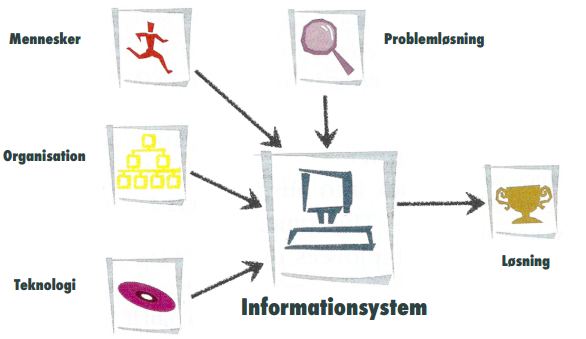
\includegraphics{images/kontekstmodel/metode.png}
  \caption[Metode for Kontekstmodellen]{Illustration af elementerne i et informationssystem. Kilde:
  \protect\citet{Laudon1999}}
  \label{fig:kontekstmodel}
\end{figure}


%\section{Informationssystem}\label{Informationssystem}
\subsection{Informationssystem}\label{subsec:Informationssystem}

Et informationssystem bruges til at effektivisere en arbejdsproces og hjælper med at holde fokus, så arbejdet
bliver gjort tilfredsstillende. Informationssystemet består af tre processor: Indsamling af data, behandling
af dataene og formidling af dataene. Der indsamles data om de tre elementer: mennesker, organisation og
teknologi. Når dataene er indsamlet, behandles de, altså der bliver analyseret på dataene. Herefter formidles
det i form af, der findes ud af, hvad datene kan bruges til. Behandlingen af de tre elementer bruges til at
finde ud af, hvad der skal tages hensyn til under problemløsningsdelen. Alt dette er et informationssystem,
som bruges til finde ud af, hvad løsningen til problemstillingen er.


%\subsection{Mennesker}\label{subsec:mennesker}
\subsubsection{Mennesker}\label{subsubsec:mennesker}

Elementet mennesker handler om personer/persongrupper, som har en interesse i, at en given problemstilling
løses. Det kan være brugeren af det program, der bliver lavet og andre, som får gavn af en løsning. Man
undersøger bl.a. brugerens evner, da programmet skal laves på en sådan måde, at brugeren har den
fornødne kunnen, til at kunne betjene programmet. Brugerens behov undersøges også, så man får alle de funktioner
med, som er nødvendige for at programmet er brugbart.


%\subsection{Organisation}\label{subsec:organisation}
\subsubsection{Organisation}\label{subsubsec:organisation}

Under organisationsafsnittet undersøges hvor og hvordan problemet opstår, derudover undersøges der hvilke regler
og værdier organisationen har, for at kunne tage disse med til problemløsningen.

\cbstart
%\subsection{Teknologi}\label{subsec:Teknologi}
\subsubsection{Teknologi}\label{subsubsec:Teknologi}

Teknologidelen omhandler de teknologier, som anvendes til at løse en informationssystem relevant problemstilling.
Ofte ville denne teknologi være en computere, servere, og internettet. Dette er altså de byggeblokke hvorpå
systemet bygges.
\cbend

%Teknologielementet handler om teknologier som allerede er på markedet, som kan løse problemstillingen. Dette
%behøver ikke kun at være løsninger som er computerbaserede, det kan også være manuelle systemer, altså hvor
%det hele gøres i hånden, med papir og blyant.


%\section{Rapportens opbygning}\label{sec:rapportens-opbygning}
\subsection{Rapportens opbygning}\label{subsec:rapportens-opbygning}

Først bliver menneskedelen behandlet, i form af en interessentanalyse, herefter vil organisationselementet blive berørt. Derefter bliver der skrevet om teknologier,
hvorefter de tre elementer munder ud i en problemafgrænsning og en problemformulering. Til sidst skrives der
om problemløsningsdelen. \fxnote{Sidste sætning skal udvides så der står hvad der vil blive skrevet om}

\chapter{Interessenter}
\section{Dansk sejlunion}
Dansk sejlunion er et forbund, som blev dannet i 1913 [http://www.sejlsport.dk/mere/dansk-sejlunion/historie]. Deres mission er at være det nationale samlingspunkt for alle sejlere. Dansk sejlunion er tilsluttet Danmarks Idrætsforbund, International Sailing Federation og andre lignende organisationer inden for sejlsport. 
Dansk sejlunion tilbyder også services i form af rådgivning og aktiviteter til klubber, sejlklasser og andre samarbejdspartnere[http://www.sejlsport.dk/mere/dansk-sejlunion/strategi-og-politik/vision-og-vaerdier].

\section{Andre fritidsklubber}

\chapter{Teknologi}\label{teknologi-analyse}

For at kunne udvikle et godt produkt der skal kunne bruges i en bådklub, er det vigtigt at se på hvilke produkter der
allerede er på markedet, altså hvad er state of the art. I denne forbindelse er der fundet forskellige produkter, som
har nogle af de features der efterspørges i et system til en bådklub. Der er f.eks. et program udviklet af Anderson
Software der hedder BoatCloud.\citep{BoatCloud} BoatCloud har lavet 3 applikationer, StackTrack, VesselValet og Service
Request. StackTrack benyttes når medlemmerne selv sejler deres både, hvorimod VesselValet, er når der skal tjenere og
passere med ombord på bådene. BoatCloud applikationerne er derfor mere designet til en bådklub, som passer på medlemmer
af klubbens egne både, fremfor klubbens egne både. I applikationerne kan medlemmerne melde at de vil sejle på et bestemt
tidspunkt. Medlemmet kan få klubben til at vaske båden, tanke den, og fylde den op med diverse snacks, alt sammen
registreres igennem denne webbaserede applikation. Applikationen tager imod alle disse bestillinger i realtime, og 24
timer i døgnet. Herudover bliver der sendt e-mails ud til medlemmerne når de har lavet en bestilling. Man kan logge ind
som administrator, og her kan man se alle reservationer der er lavet, samt har man mulighed for at se yderligere
detaljer om hver enkelt reservation.

En anden applikation der findes er Sailing Club Manager. \citep{SailClub} Denne applikation er også webbaseret, og gør
det muligt for en bådklub at tilføje hvilke både der er samt hvor det er fortøjnet i marinen. Man kan i en kalender
lave events, og bookninger, her kan medlemmerne så melde sig på de forskellige events. Applikationen kan også bruges som
kontaktmedium for klubben til deres medlemmer. Klubben kan sætte et mail system op, samt tilføje et template som bliver
sendt med hver enkelt mail. Applikationen kan endvidere holde styr på økonomien, man kan tilføje en bankkonto, samt kan
det holde styr på fakturaer, og endda sende dem og håndtere det online. Man kan tilføje medlemsskaber, med forskellige
oplysninger omkring medlemmerne der har netop dette medlemsskab i klubben.

Ud fra denne undersøgelse er flg. features altså fundet i applikationerne:

\begin{itemize}
	\item Medlemmer kan booke afgange.
	\item Medlemmer kan melde sig på events i bådklubben.
	\item Medlemmer kan betale igennem hjemmesiden.
	\item Medlemmerne kan bede klubben om at gøre deres egen båd klar, med forskellige aftaler klubben håndterer før den aftalte tid.
	\item Bådklubben kan vise hvilke både der er i klubben.
	\item Bådklubben kan oprette events, og afsætte hvilke medlemmer der kan melde sig på eventet.
	\item Bådklubben kan oprette forskellige medlemsskaber og opkræve betalinger igennem hjemmesiden.
	\item Bådklubben kan sende e-mails med klubbens egne templates gennem hjemmesiden, herunder påmindelser om en bookning nogen tid før.
\end{itemize}

\fxnote{Hvad kan vi konkludere ud fra dette ? Skal vi skrive at vi vil konkludere på det i et problemafgrænsnings afsnit ? Jeg tænker noget i stil med hvilke features vores egen applikation skal have, samt hvilke features vi skal have udover dette, som vi er kommet frem til i forbindelse med organisations afsnittet :) ?}
\chapter{Organisation}\label{chap:organisation}

\cbstart

\section{Sejlklubben Sundet}

I Sejlklubben Sundet findes flere både, af forskellig størrelse, som bruges til undervisning af klubbens
elever, såvel som udlån til klubbens medlemmer.

Undervisningen foregår hen over hverdagene, hvorimod bådudlån foregår i weekenderne. En enkelt klasse af både
kan dog også udlånes om onsdagen.

For at måtte sejle skal der være minimum én fører med i bådens besætning \fxnote{Husk at definere fører og
muligvis besætning, hvis dette bibeholdes.}. Desuden bestemmes prisen for udlånet bl.a. efter besætning også,
idet tilstedeværelsen af en af klubbens elever gør, at udlånet er gratis.

Håndteringen af de forskellige data blev, og bliver muligvis stadig, udført på papir, ved manuelt arbejde,
hvilket ifølge oplysninger \fxnote{Muligvis angive en mere officiel kilde her?} kan resultere i, at det kun
bliver gjort engang imellem.

Ved et kig på Sejlklubben Sundets hjemmeside \citep{SundetUdlaan} ses det, at forskellige værktøjer er taget i
brug, i et forsøg på at øge brugervenlighed og interaktion mellem deltagere. Det er på nuværende tidspunkt
uvist, hvor vidt disse tiltag har haft den ønskede, gavnlige effekt.

\cbend


%\part{Problemløsning}

%\chapter{Eksempler}

{\itshape Dette dokument er primært ment som en hjælp til at se de forskellige muligheder
i rapporten.}

\section{Akronymer}
For lettere at håndtere akronymer, benyttes en pakke, hvor disse defineres én gang, og bruges så i
dokumentet ved hjælp af \textbackslash ac{acronym}. Så vil systemet sørge for, at skrive det fuldt
ud første gang man eksempelvis skriver \ac{AAU} eller \ac{KOT}.

Skulle det derefter ske, at man har behov for at snakke om \ac{AAU} igen, vil den bruge forkortelsen,
og dermed selv holde styr på det. Dette sikrer os bedre mod fejl. :)

\section{Ændringsregistreringer}
For at lette kommunikation med vejleder kan vi registrere ændringer på forskellige måder.

\subsection{Hele afsnit}
\cbstart Man kan markere, at et helt afsnit er blevet ændret eller tilføjet, ved hjælp af kommandoerne
\textbackslash cbstart og \textbackslash cbend, som markerer henholdsvist start og slut på sidebaren.\cbend

Det er også muligt at markere, at noget er blevet slettet, med \textbackslash cbdelete, hvilket er gjort i
dette \cbdelete afsnit.

\subsection{Detaljerede ændringer}
Der er også mulighed for at vise mere detaljerede ændringer. Eksempelvis \added[id=TB]{hvis man tilføjer tekst},
eller \deleted[id=TB]{sletter tekst}. Eller for den sags skyld \replaced[id=TB]{en kombination af de to}{a
combination of the two}.

\section{Matematik}
Matematiske formler er lette at indsætte\ldots

\begin{equation} \label{eq:example}
  f\left(x\right) = \dfrac{a \cdot b}{c}
\end{equation}

\section{ToDo--typer}
Der er fire forskellige typer af noter, og brugen heraf bestemmes af gruppen i fællesskab, så der er enighed om,
hvad der benyttes til hvilket.

\subsection{Generelt}
Først og fremmest er der noterne almindelig\fxnote{Peger på et bestemt sted i teksten.}
og \fxnote*{Fremhæver et tekststykke også.}{med modtagertekst}.

Ligeledes er der advarsler\fxwarning{Dette er en advarsel!} og fejl\fxerror{Dette er en fejl!}. Sidstnævnte
vil desuden forhindre dokumentet i at kompilere, hvis det markeres som værende \emph{final}.

Disse tre typer kan naturligvis også bruges i \emph{stjerneformen}, til at fremhæve et bestemt stykke
tekst som denne tilknyttes.

\subsection{Avanceret}
Til de lidt mere krævende noter kan det være nødvendigt med mere tekst, hvilket kræver et environment.

\begin{anfxnote}{Dette er en opsummering.}
Dette kan benyttes til at få nogle længere noter ind i teksten, hvis der eksempelvis er noget der skal
overvejes, hvor det bare ikke er nok men en lille notits.

Foruden denne anfxnote er der også \emph{anfxwarning}, \emph{anfxerror} og \emph{anfxfatal}, ligesom ovenfor.
\end{anfxnote}


\section{Referencer}
Det er muligt at referere til forskellige ting, eksempelvis kan nævnes \myref{eq:example}.

For at oprette en såkaldt \emph{label}, som senere kan refereres til, benyttes \verb|\label{key}|. Det er god
stil indenfor \LaTeX at benytte prefixes til de forskellige labels, eksempelvis:
\begin{table}[h]
  \begin{center}
    \begin{tabular}{ll}
      \toprule[1.5pt]
      \texttt{chap:}   & chapter              \\ 
      \texttt{sec:}    & section              \\ 
      \texttt{subsec:} & subsection           \\ 
      \texttt{fig:}    & figure               \\ 
      \texttt{tab:}    & table                \\ 
      \texttt{eq:}     & equation             \\ 
      \texttt{lst:}    & code listing         \\ 
      \texttt{itm:}    & enumerated list item \\ 
      \texttt{ex:}     & example              \\
      \bottomrule[1.5pt]
    \end{tabular}
  \end{center}
  \caption{Reference prefixes} \label{tab:reference_prefixes}
\end{table}


\section{Eksempelbokse}

\begin{example}{Overskrift}
  \label{ex:an_example}
  \lipsum[1]
\end{example}



\section{Programmeringskode}




%%%%%%%%%%%%%%%%
%% REFERENCES %%
%%%%%%%%%%%%%%%%

%\backmatter
\makeatletter\@openrightfalse
\let\cleardoublepage\clearpage
\part{Referencer}

%%% Bibliography %%%
\bibliography{bibtex/litteratur}

%%% Figures %%%
\newpage
\listoffigures

%%% Tables %%%
\listoftables


\@openrighttrue\makeatother


%%%%%%%%%%%%%%
%% APPENDIX %%
%%%%%%%%%%%%%%

\part{Appendiks}
\appendix
\settocdepth{chapter}

% Insert each appendix under this



%%%%%%%%%
% INDEX %
%%%%%%%%%

\newpage
\printindex

\end{document}
